\chapter{One Engine Before Many Buckets}

This chapter follows a School of Hard Knocks interview with Grant Mitt, founder of Mitt Group. It is not a blackboard lecture, but it does have a mathematical spine: base rates, thresholds, follower counts, recruiting percentages, scaling comparisons, and simple resource accounting. We should read the numbers as interview claims rather than audited statistics. Their purpose is to make entrepreneurship less vague. The lecture's movement is disciplined: enter the market without hiding behind age, look at the odds, concentrate before diversifying, use media as leverage, earn confidence through sales, scale through people, and protect the energy that lets the whole system keep running.

\section{The Market Does Not Care About Age}

The first question is about confidence. Mitt is young, and the host asks how a young founder can compete in an industry where owners and decision makers may be much older. Mitt's answer is not inspirational in the usual sense. It is almost mechanical: if we make age the decisive variable, other people will treat it that way too; if we do not, the market still has to judge the offer.

His analogy is the NFL. Once a player is in the league, a rookie and a nineteen-year veteran can both be cut, both can win, and both can compete. The corresponding business claim is that once we are actually attacking the market, the relevant question is not age by itself. It is whether the market chooses to transact.

Let \(M\) denote the market's selection mechanism. Mitt's point can be written as a warning against using the wrong explanatory variable:
\begin{equation}
  \hbox{market result}
  \approx
  M(\hbox{offer},\hbox{execution},\hbox{trust}),
  \qquad
  \hbox{not simply } M(\hbox{age}).
\end{equation}

This is not a formal model of buyer behavior. It is an operator's correction. If the first explanation for a lost deal is ``I am too young,'' attention leaves the things that can actually be improved: the offer, the execution, and the trust signal.

\section{Why Start When The Base Rates Are Bad?}

The next pivot is sharper. The host asks when Mitt decided not to follow the corporate route. Mitt answers first with necessity: people depended on him, and he felt he had to act. But he immediately resists the easy story that starting a business is automatically the brave or wealth-building path.

In the interview, he gives two base-rate claims:
\begin{align}
  \Pr(\hbox{company breaks even or loses money})
    &\approx 0.86,\\
  \Pr(R_{\hbox{company}}>\$10{,}000{,}000)
    &\approx 0.005.
\end{align}
Here \(R_{\hbox{company}}\) means company revenue. These are Mitt's spoken figures: roughly \(86\%\) of companies break even or lose money, and roughly one half of one percent ever pass ten million dollars in revenue.

He also compares the average business owner with the average employee. The transcript gives the rough comparison as ``58 to 55'' and says that the employee makes about \(\$3{,}000\) to \(\$4{,}000\) more. The safest notation keeps the unit cautious:
\begin{equation}
  \bar I_{\hbox{employee}}
  -
  \bar I_{\hbox{business owner}}
  \approx
  \$3{,}000\hbox{ to }\$4{,}000.
\end{equation}
The numerical precision is not the point. The point is that ownership alone is not wealth. The base rates make entrepreneurship a conditional choice, not an identity.

\subsection{Question \& Answer}

\paragraph{Question.}
Should everyone start a business if they want to build wealth?

\paragraph{Answer.}
No. Mitt's answer is that the choice is not simply employment versus entrepreneurship. A person may be an employee, an intrapreneur, or an entrepreneur. The intrapreneur builds wealth and responsibility inside a strong company that gives real room to grow. Mitt says that people inside Mitt Group can become multimillionaires that way, provided the company is structured to create that opportunity.

The decision space is therefore:
\begin{equation}
  \hbox{path}
  \in
  \{\hbox{employee},\hbox{intrapreneur},\hbox{entrepreneur}\}.
\end{equation}

\begin{table}
\centering
\begin{tabular}{p{0.27\linewidth}p{0.30\linewidth}p{0.33\linewidth}}
\hline
Path & Main upside & Necessary condition \\
\hline
Employee &
Stable role and income &
Accepts limited ownership upside \\
Intrapreneur &
Upside inside a strong firm &
Company must create real room \\
Entrepreneur &
Direct ownership and control &
Operator bears direct downside \\
\hline
\end{tabular}
\caption{The interview's three-path distinction. The table reconstructs Mitt's spoken contrast between employment, intrapreneurship, and entrepreneurship.}
\end{table}

Mitt's own case is then not generalized into a rule for everyone. He says he had the time, the resources, the capital, and the preparation. He also says he was willing to lose every penny knowing that he had tried. That willingness matters because it separates necessity from casual aspiration.

\section{Concentration Before Diversification}

The host then asks about diversification. This is one of the central turns in the lecture. Mitt does not argue that diversification is always bad. He argues that it is usually premature. If the first engine has not yet produced a meaningful surplus, then diversification may simply mean being average at several things.

Mitt's own threshold was the solar business:
\begin{equation}
  R_{\hbox{solar}}>\$10{,}000{,}000
  \quad\Longrightarrow\quad
  \hbox{diversification can begin}.
\end{equation}
This should be read as his sequence, not as a universal law. He says he did not start diversifying until the solar company was over ten million dollars in revenue. Even then, most of his focus and energy stayed with solar.

\subsection{Question \& Answer}

\paragraph{Question.}
If millionaires often have several income streams, why not build several streams immediately?

\paragraph{Answer.}
Mitt's answer is that the streams are often the result, not the cause. In his phrasing, we first make the big pile. Then we allocate from it into buckets that can produce more money. If there is no big pile, there is often nothing meaningful to allocate, and the operator risks becoming kind of good at many things and great at none.

\begin{figure}
\centering
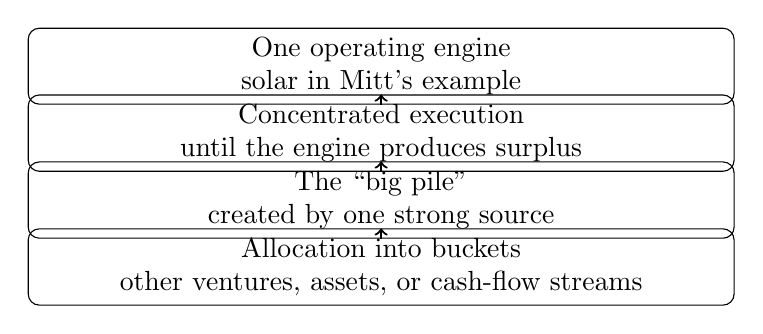
\begin{tikzpicture}[
  node distance=0.85cm,
  box/.style={draw, rounded corners, align=center,
              text width=0.72\linewidth, minimum height=0.85cm},
  arrow/.style={->, thick}
]
\node[box] (engine) {One operating engine\\solar in Mitt's example};
\node[box, below of=engine] (execution) {Concentrated execution\\until the engine produces surplus};
\node[box, below of=execution] (pile) {The ``big pile''\\created by one strong source};
\node[box, below of=pile] (allocation) {Allocation into buckets\\other ventures, assets, or cash-flow streams};
\draw[arrow] (engine) -- (execution);
\draw[arrow] (execution) -- (pile);
\draw[arrow] (pile) -- (allocation);
\end{tikzpicture}
\caption{The concentration-before-diversification sequence reconstructed from the interview.}
\end{figure}

The transcript also contains projected revenue language. Mitt says the solar company will ``revenue 30 this year'' and then ``90, 120'' next year. The likely unit is millions of dollars, but the sentence does not explicitly state the unit. A cautious note records the claims as:
\begin{equation}
  R_{\hbox{solar,this year}}\approx 30,
  \qquad
  R_{\hbox{solar,next year}}\approx 90\hbox{ to }120,
\end{equation}
with the unit treated as inferred from context rather than directly stated.

\section{Media As Leverage Around The Main Business}

Only after concentration does the interview turn to content. That order matters. Mitt does not present social media as another scattered hustle. He presents it as leverage around the main operating business: credibility, recruiting, connections, and brand.

The host frames Mitt as having a following above \(100{,}000\). Mitt gives more specific counts:
\begin{equation}
  F_{\hbox{TikTok}}\approx 145{,}000,
  \qquad
  F_{\hbox{Instagram}}\approx 25{,}000.
\end{equation}
He then gives a recruiting example. In a company-wide meeting with several new starters, he says that \(30\%\) to \(40\%\) of them reported that they had followed him or discovered the company through social media:
\begin{equation}
  \Pr(\hbox{new starter linked to Grant's social presence})
  \approx
  0.30\hbox{ to }0.40.
\end{equation}

This gives the chapter a useful distinction. Media is not only a sales channel. It expands the surface area of trust. People hear about the company, understand the founder, and sometimes become employees. Mitt also says that appearances on Fox Business and similar opportunities would not necessarily have happened even if the company were ten times bigger. They happened because the individual brand existed.

As a schematic, not a strict identity, we can write:
\begin{equation}
  \hbox{media leverage}
  \sim
  \hbox{trust}
  +
  \hbox{reach}
  +
  \hbox{recruiting surface}.
\end{equation}
The important word is leverage. The content is valuable because it compounds the main business, not because it replaces it.

\section{Risk, Sales, And Learned Confidence}

The next question is risk. Mitt starts broadly: risk-taking is everything. But he immediately qualifies the sentence. There are times to be risk-on and risk-off; one should prepare for a rainy day; one has to be smart. The deeper claim is that risk becomes less reckless when it is backed by earned capability.

His examples are vivid. He does not want to wait until age seventy-five to enjoy the results of risk. He would rather build while the payoff can still affect his life and his family. Then he gives the Sahara Desert image: if everything were taken away but his mind and capabilities remained, he believes he could rebuild faster because he now knows what to do.

The mechanism is:
\begin{equation}
  \hbox{comfort with risk}
  \uparrow
  \quad\hbox{as}\quad
  \hbox{earned capability and self-trust}
  \uparrow.
\end{equation}

Mitt defines self-trust operationally. It comes from keeping promises to oneself and executing when things get hard. Let \(C_t\) denote confidence at time \(t\), not as mood but as an internal estimate of execution reliability. A simple update rule is:
\begin{equation}
  C_{t+1}
  =
  C_t
  +
  \alpha P_t
  -
  \beta B_t,
  \qquad
  \alpha,\beta>0.
\end{equation}
Here \(P_t=1\) when a promise is kept and \(B_t=1\) when a promise is broken. The equation is a reconstruction of the mechanism, not a transcript quotation. It captures the idea that confidence is not merely asserted; it is updated by evidence.

\subsection{Question \& Answer}

\paragraph{Question.}
Why can't sales skill be learned from a textbook?

\paragraph{Answer.}
Because the relevant skill is not just knowing what to say. Mitt says experience cannot be Googled. A person has to be told no, cursed out, rejected repeatedly, and still deliver the message correctly. The lesson is empirical.

A compact learning loop is:
\begin{align}
  \hbox{attempt}_{t}
    &\longrightarrow
  \hbox{customer response}_{t},\\
  \hbox{customer response}_{t}
    &\longrightarrow
  \hbox{adjusted message}_{t+1},\\
  \hbox{many repetitions}
    &\longrightarrow
  \hbox{judgment}.
\end{align}

Mitt's example is selling DirecTV inside Walmart when he was eighteen or nineteen. People were buying bread, tired from work, annoyed, or uninterested. That environment forced adaptation. In the lecture's logic, sales is not a side skill. It is one of the ways an operator learns what reality will and will not accept.

\section{Scaling Means People, Not Gadgets}

The sales discussion leads naturally into scaling. Before the abstract rule, there is a concrete count. The host asks how many states Mitt Group is closing solar deals in. Mitt answers:
\begin{equation}
  N_{\hbox{states}}=17.
\end{equation}

Then he defines scaling. Scaling is doing the little things right at scale. The warning is that people often try to expand before they have conquered one place. They ask whether to enter Europe or another city before they are winning where they already are.

The crucial contrast is between incremental improvement and real scale. Mitt says a CRM, a new technology, or one smart hire may improve the business by \(10\%\) or \(20\%\), but it will not by itself double, triple, or quadruple revenue:
\begin{equation}
  \Delta_{\hbox{tool}}
  \approx 10\%\hbox{ to }20\%,
  \qquad
  \Delta_{\hbox{scale}}
  \in
  \{2\times,3\times,4\times,\ldots\}.
\end{equation}

\paragraph{Worked scaling comparison.}
Suppose current revenue is \(R_0\). A strong tool improvement of \(20\%\) gives
\begin{equation}
  R_1=1.20R_0.
\end{equation}
Tripling revenue would require \(3R_0\). The gap between a \(20\%\) improvement and a tripling is
\begin{equation}
  3R_0-1.20R_0=1.80R_0.
\end{equation}
In Mitt's account, that missing \(1.80R_0\) is not supplied by the tool alone. It comes from trained people executing fundamentals without the founder doing everything for them.

\begin{table}
\centering
\begin{tabular}{p{0.28\linewidth}p{0.30\linewidth}p{0.32\linewidth}}
\hline
Scaling input & Transcript claim & Mechanism \\
\hline
CRM or technology &
May add \(10\%\) to \(20\%\) &
Improves process efficiency \\
One smart hire &
Helpful but insufficient alone &
Adds local capability \\
Many trained people &
Required for real scale &
Distributes execution \\
Founder oversight &
Cannot cover everything &
Must become systems and standards \\
\hline
\end{tabular}
\caption{Incremental improvement versus true scale in Mitt's operating account.}
\end{table}

The phrase ``scaling is people'' is the center of this section. A billion-dollar company, in Mitt's framing, requires thousands of people who know what they are doing, including people as smart as or smarter than the founder in particular domains.

\section{Energy, Industry Choice, And The Hiring Filter}

The final movement turns from scale to endurance. The host asks how Mitt avoids burnout. Mitt answers with a resource model. We wake up with a certain amount of energy. Every communication, interaction, and decision drains some of it. The word ``no'' becomes important because attention is scarce.

Let \(E_0\) be the available energy at the start of the day, and let interaction \(i\) consume \(c_i\). A simple accounting model is:
\begin{equation}
  E_{\hbox{remaining}}
  =
  E_0-\sum_i c_i.
\end{equation}
The point is not physiology. It is operating control. If one appointment goes badly and the operator spends energy being angry, that cost enters the next appointment. Mitt's practical rule is to stay level-headed through highs and lows, manage emotion, and protect consistency.

The industry-choice question comes next. Mitt says that around 2014--2016 he was looking for industries likely to be bigger in twenty years than they were then: technology, AI, robotics, renewable energy, and crypto. He did not claim mastery at the beginning. He wanted a growing arena where he could get a foot in the door, learn, and build.

That gives us another compact reconstruction:
\begin{equation}
  \hbox{good arena}
  \sim
  \hbox{future growth}
  +
  \hbox{room to enter}
  +
  \hbox{chance to learn}.
\end{equation}

The last substantive answer is about hiring. Mitt's non-negotiables are coachability, humility, and persistence. He explicitly says that talent at another company is not enough. Talent proves there is ability; it does not prove that the person will succeed here. He also adds the harder filter of necessity: people with a comfortable fallback often do not push through in the same way as people who have to make it work.

\begin{equation}
  \hbox{hire}
  \Longleftarrow
  \hbox{coachable}
  \wedge
  \hbox{humble}
  \wedge
  \hbox{persistent}
  \wedge
  \hbox{no easy fallback}.
\end{equation}

The notation is schematic, but the sequence is faithful. The business chooses an arena, concentrates on one engine, scales through people, and then selects for the traits that let those people survive the pressure of the arena.

\section{Summary}

The lecture's entrepreneurship lesson is a sequence of filters. First, remove age as the central excuse and let the market test the offer. Second, judge entrepreneurship against base rates rather than romance; employment, intrapreneurship, and ownership are distinct paths. Third, concentrate before diversifying: make the big pile before allocating into buckets. Fourth, use media as leverage around the main business, especially for credibility and recruiting. Fifth, understand risk as something earned through capability, repetition, and self-trust. Sixth, scale through people who can execute fundamentals without constant founder oversight. Finally, protect energy, choose growing arenas, and hire for coachability, humility, persistence, and necessity.